\documentclass[tikz,border=10pt]{standalone}
\usepackage{tikz}
% Aggiunta la libreria 'shadows' necessaria per l'opzione drop shadow
\usetikzlibrary{shapes, arrows.meta, calc, backgrounds, positioning, patterns, shadows}
% -------- PALETTE COLORI --------

% 1. Famiglia L^p (Toni del BLU/AZZURRO - FREDDI)
\definecolor{L1loc}{RGB}{215, 235, 250}   % Azzurro chiarissimo (sfondo ampio)
\definecolor{L1col}{RGB}{130, 190, 255}   % Ciano deciso
\definecolor{L2col}{RGB}{100, 160, 240}   % Blu reale chiaro
\definecolor{Linfcol}{RGB}{70, 130, 200}  % Blu acciaio

% 2. Famiglia H^s (Toni del VIOLA/AMETISTA - NUOVO CONTRASTO)
% Questi colori staccano nettamente dal blu degli L^p
\definecolor{H1col}{RGB}{210, 160, 240}   % Lilla/Orchidea
\definecolor{Hscol}{RGB}{160, 100, 220}   % Viola acceso

% 3. Famiglia C^k (Toni dell'ARANCIO/OCRA - CALDI)
\definecolor{C0col}{RGB}{255, 240, 200}   % Crema
\definecolor{C1col}{RGB}{255, 215, 160}   % Pesca
\definecolor{Ckcol}{RGB}{250, 190, 120}   % Ocra chiaro
\definecolor{Cinfcol}{RGB}{240, 160, 100} % Arancio

% 4. Distribuzioni e Supporti Compatti
\definecolor{Scol}{RGB}{255, 200, 220}      % Rosa (Schwartz)
\definecolor{Sprimecol}{RGB}{230, 210, 230} % Grigio-viola (S')
\definecolor{Eprimecol}{RGB}{200, 230, 180} % Verde oliva chiaro (E')

% 5. Intersezione e Delta
\definecolor{C0infcol}{RGB}{255, 255, 150}  % Giallo Limone (Cuore)
\definecolor{Deltacol}{RGB}{220, 80, 80}    % Rosso (Dirac)

% Sfondo
\definecolor{Bgcol}{RGB}{250, 250, 250}
\definecolor{Bgdraw}{RGB}{180, 180, 180}

\begin{document}

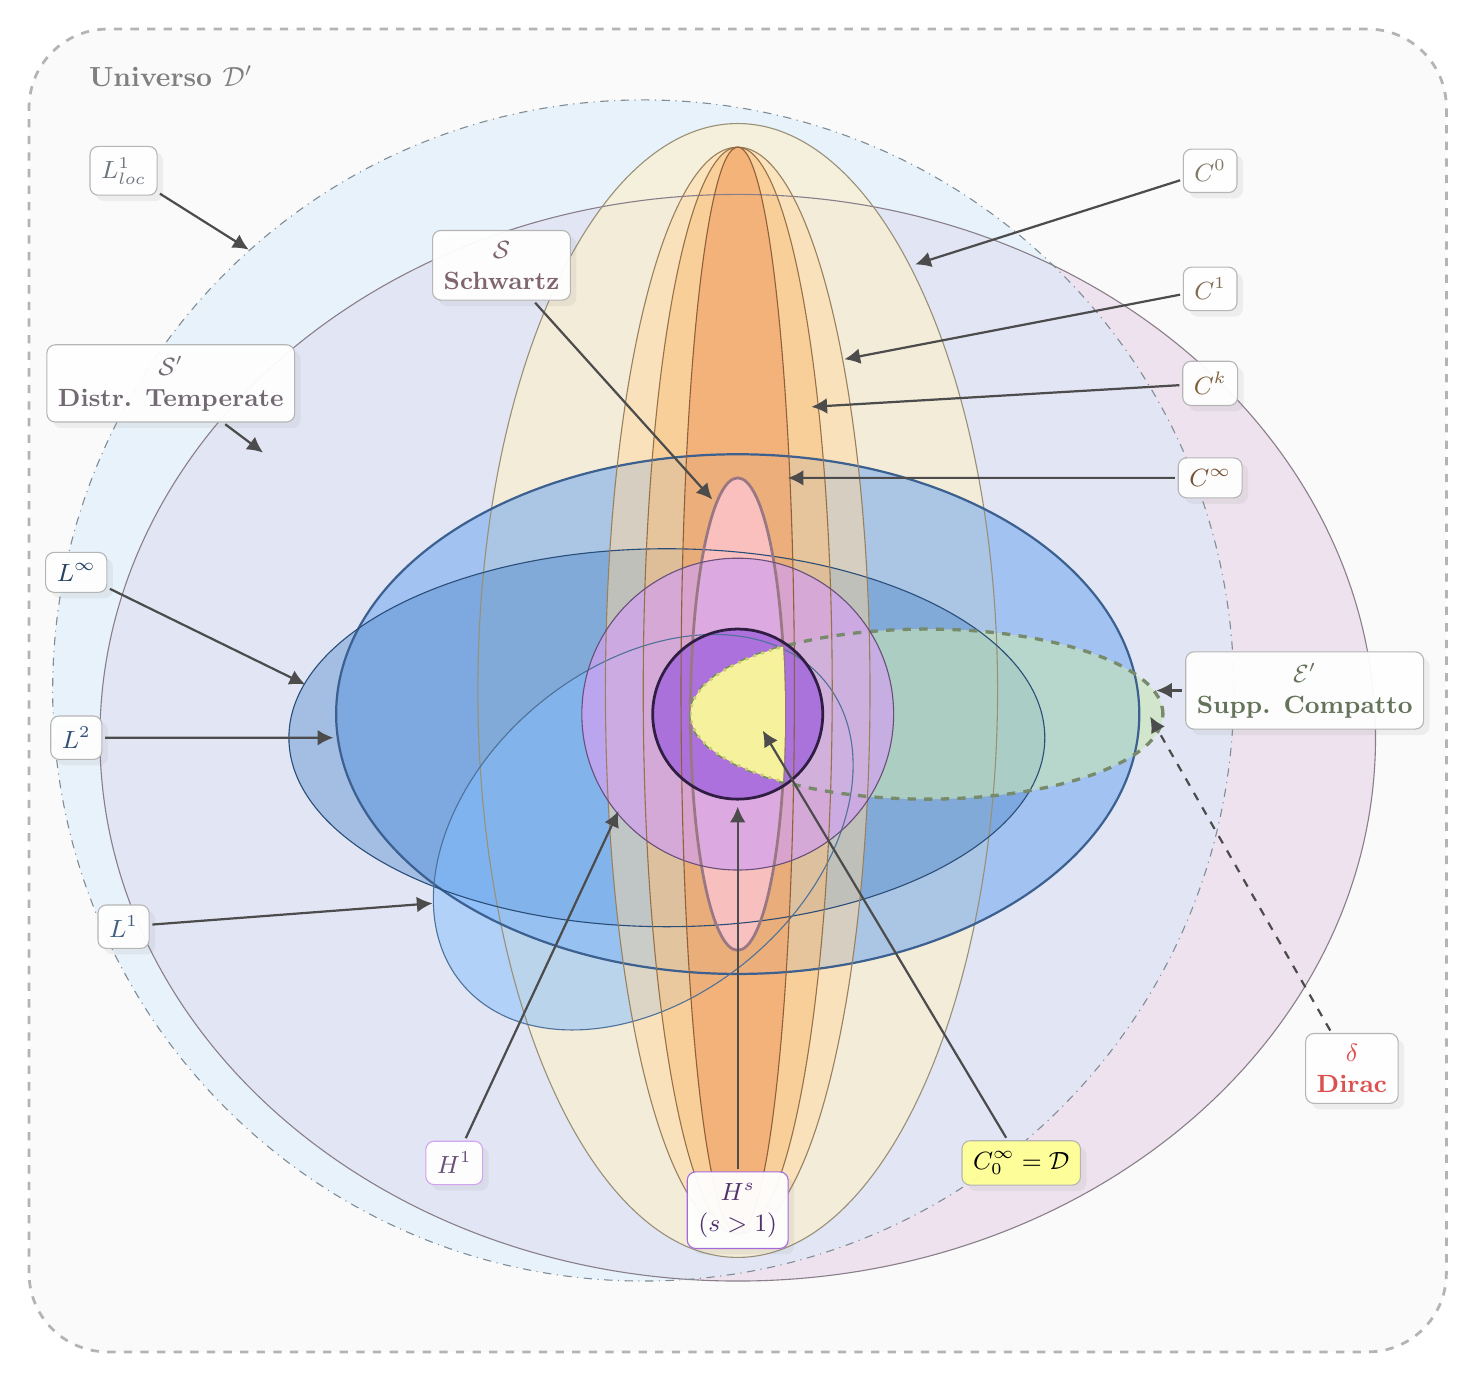
\begin{tikzpicture}[
    scale=0.6, 
    every node/.style={align=center},
    labelbox/.style={
        rectangle, rounded corners=3pt,
        draw=black!30, fill=white,
        inner sep=4pt, font=\small\bfseries,
        drop shadow={opacity=0.1},
        opacity=0.95, text opacity=1
    },
    arrowstyle/.style={
        -{Latex[length=2mm, width=2mm]}, 
        line width=0.8pt,
        color=black!70,
        shorten >=1pt, shorten <=1pt
    }
]

    % Definizioni forme geometriche ricorrenti
    \def\pathS{(0,-0.5) ellipse (1.0 and 5.0)}
    \def\pathEprime{(4,-0.5) ellipse (5 and 1.8)}

    % ------------------- RIEMPIMENTI (LAYER INFERIORI) -------------------

    % Universo D' (Sfondo rettangolare arrotondato)
    \fill[Bgcol, rounded corners=1cm] (-15,-14) rectangle (15,14);

    % S' (Distribuzioni Temperate) - Grande ellisse
    \fill[Sprimecol, opacity=0.6] (0,-1) ellipse (13.5 and 11.5);

    % L^1_loc - Ellisse leggermente più piccola ma ampia
    \fill[L1loc, opacity=0.5] (-2,0) ellipse (12.5 and 12.5);

    % C^0 (Continue)
    \fill[C0col, opacity=0.6] (0,0) ellipse (5.5 and 12);

    % L^2 (Spazio di Hilbert) - Ellisse orizzontale
    \fill[L2col, opacity=0.5] (0,-0.5) ellipse (8.5 and 5.5);

    % L^inf - Ellisse spostata a sinistra
    \fill[Linfcol, opacity=0.4] (-1.5,-1) ellipse (8.0 and 4.0);

    % L^1 - Ellisse ruotata in basso a sinistra
    \fill[L1col, opacity=0.5, rotate around={40:(-2,-3)}] (-2,-3) ellipse (5 and 3.5);

    % --- Famiglia C nested ---
    % C^1
    \fill[C1col, opacity=0.5] (0,0) ellipse (2.8 and 11.5);
    % C^k
    \fill[Ckcol, opacity=0.5] (0,0) ellipse (2.0 and 11.5);
    % C^inf
    \fill[Cinfcol, opacity=0.6] (0,0) ellipse (1.2 and 11.5);

    % S (Schwartz)
    \fill[Scol, opacity=0.7] \pathS;

    % E' (Supporto compatto)
    \fill[Eprimecol, opacity=0.6] \pathEprime;

    % --- Spazi Sobolev (H) - Colori VIOLA per contrasto ---
    % H^1
    \fill[H1col, opacity=0.7] (0,-0.5) circle (3.3);
    % H^s
    \fill[Hscol, opacity=0.8] (0,-0.5) circle (1.8);

    % ------------------- BORDI E DETTAGLI -------------------

    % Bordo Universo
    \draw[Bgdraw, dashed, line width=1pt, rounded corners=1cm] (-15,-14) rectangle (15,14);

    % Contorni principali
    \draw[Sprimecol!60!black] (0,-1) ellipse (13.5 and 11.5);
    \draw[L1loc!60!black, dash dot] (-2,0) ellipse (12.5 and 12.5);
    \draw[C0col!60!black] (0,0) ellipse (5.5 and 12);
    
    \draw[L2col!60!black, line width=0.8pt] (0,-0.5) ellipse (8.5 and 5.5);
    \draw[Linfcol!60!black] (-1.5,-1) ellipse (8.0 and 4.0);
    \draw[L1col!60!black, rotate around={40:(-2,-3)}] (-2,-3) ellipse (5 and 3.5);

    \draw[C1col!60!black] (0,0) ellipse (2.8 and 11.5);
    \draw[Ckcol!60!black] (0,0) ellipse (2.0 and 11.5);
    \draw[Cinfcol!60!black] (0,0) ellipse (1.2 and 11.5);
    
    \draw[Scol!60!black, line width=1pt] \pathS;
    \draw[Eprimecol!60!black, dashed, line width=1.2pt] \pathEprime;

    % Intersezione S ∩ E' (Cuore C0_inf) - Disegnato sopra gli H per visibilità
    \begin{scope}
        \clip \pathS;
        \fill[C0infcol, opacity=0.9] \pathEprime; % Giallo brillante
        \draw[C0infcol!80!black, dotted, line width=1pt] \pathEprime;
    \end{scope}

    % Contorni H (Sobolev)
    \draw[H1col!50!black] (0,-0.5) circle (3.3);
    \draw[Hscol!30!black, line width=1pt] (0,-0.5) circle (1.8);

   % ------------------- LABELS (L^2 e L^inf a Sinistra) -------------------

    % --- QUADRANTE ALTO SINISTRA ---
    \node[text=gray, font=\bfseries] at (-12, 13) {Universo $\mathcal{D}'$};
    
    \node[labelbox, text=L1loc!50!black] (lL1loc) at (-13, 11) {$L^1_{loc}$};
    \draw[arrowstyle] (lL1loc) -- (-10.3, 9.3);

    \node[labelbox, text=Sprimecol!50!black] (lSprime) at (-12, 6.5) {$\mathcal{S}'$\\Distr. Temperate};
    \draw[arrowstyle] (lSprime) -- (-10, 5);

    % --- NUOVO BLOCCO SINISTRA (Spazi L impilati) ---
    
    % L^infty (Spostato a sinistra)
    \node[labelbox, text=Linfcol!50!black] (lLinf) at (-14, 2.5) {$L^\infty$};
    \draw[arrowstyle] (lLinf) -- (-9.1, 0.1);

    % L^2 (Spostato a sinistra)
    \node[labelbox, text=L2col!50!black] (lL2) at (-14, -1.0) {$L^2$};
    \draw[arrowstyle] (lL2) -- (-8.5, -1.0);

    % L^1 (Spostato leggermente più in basso per fare spazio)
    \node[labelbox, text=L1col!50!black] (lL1) at (-13, -5) {$L^1$};
    \draw[arrowstyle] (lL1) -- (-6.4, -4.5);


    % --- QUADRANTE ALTO DESTRA (Famiglia C) ---
    \node[labelbox, text=C0col!50!black] (lC0) at (10, 11) {$C^0$};
    \draw[arrowstyle] (lC0) -- (3.7, 9);
    
    \node[labelbox, text=C1col!50!black] (lC1) at (10, 8.5) {$C^1$};
    \draw[arrowstyle] (lC1) -- (2.2, 7);
    
    \node[labelbox, text=Ckcol!50!black] (lCk) at (10, 6.5) {$C^k$};
    \draw[arrowstyle] (lCk) -- (1.5, 6);
    
    \node[labelbox, text=Cinfcol!50!black] (lCinf) at (10, 4.5) {$C^\infty$};
    \draw[arrowstyle] (lCinf) -- (1.0, 4.5);


    % --- CENTRO ALTO (Schwartz) ---
    \node[labelbox, text=Scol!50!black] (lS) at (-5, 9) {$\mathcal{S}$\\Schwartz};
    \draw[arrowstyle] (lS) -- (-0.5, 4);


    % --- QUADRANTE BASSO DESTRA (Solo E') ---
    \node[labelbox, text=Eprimecol!50!black] (lEprime) at (12, 0) {$\mathcal{E}'$\\Supp. Compatto};
    \draw[arrowstyle] (lEprime) -- (8.8, 0);


    % --- CENTRO BASSO (Sobolev) ---
    \node[labelbox, draw=H1col, text=H1col!50!black] (lH1) at (-6, -10) {$H^1$};
    \draw[arrowstyle] (lH1) -- (-2.5, -2.5);
    
    \node[labelbox, draw=Hscol, text=Hscol!50!black, font=\small\bfseries] (lHs) at (0, -11) {$H^s$\\$(s > 1)$};
    \draw[arrowstyle] (lHs) -- (0, -2.4);


    % --- CENTRO (Cuore e Dirac) ---
    \node[labelbox, fill=C0infcol, text=black] (lC0inf) at (6, -10) {$C_0^\infty = \mathcal{D}$};
    \draw[arrowstyle] (lC0inf) -- (0.5, -0.8);
    
    \node[labelbox, text=Deltacol] (lDelta) at (13, -8) {$\delta$\\Dirac};
    \draw[arrowstyle, dashed] (lDelta) -- (8.7, -0.5);
\end{tikzpicture}
\end{document}